\documentclass[tikz]{standalone}
\usepackage{tikz}

\definecolor{codeblue}{RGB}{69, 161, 248}
\definecolor{codegray}{RGB}{40, 40, 40}
\usetikzlibrary{shapes,arrows}
\tikzstyle{decision} = [diamond, draw, fill=codegray, text=white,
    text width=4.5em, text badly centered, node distance=3cm, inner sep=0pt]
\tikzstyle{block} = [rectangle, draw, fill=codeblue,  text=white,
    text width=5em, text centered, rounded corners, minimum height=4em]
\tikzstyle{line} = [draw, -latex']


\begin{document}
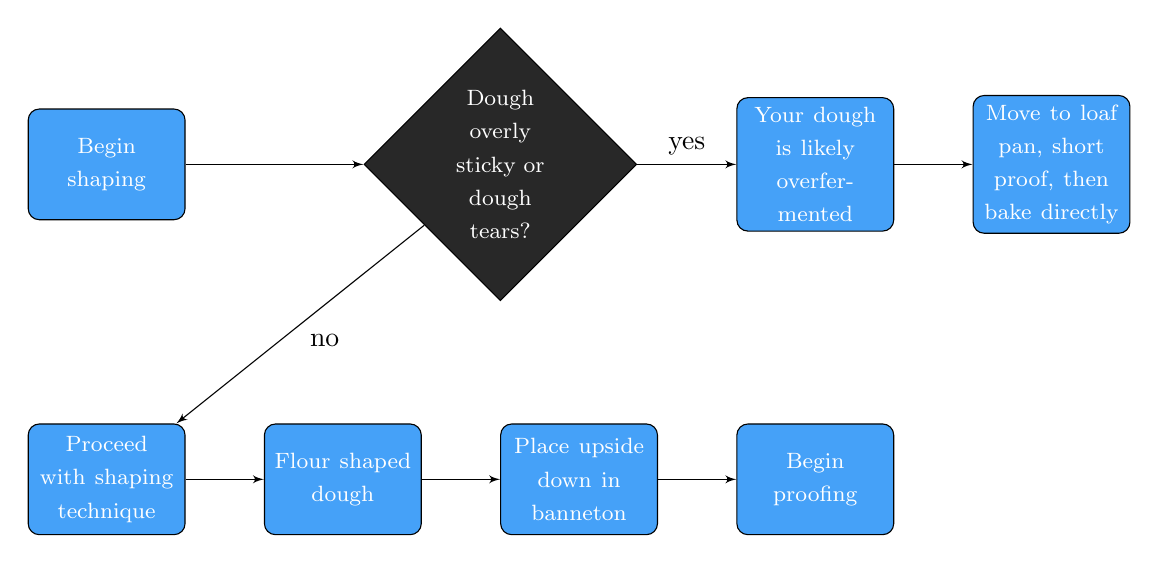
\begin{tikzpicture}[node distance = 3cm, auto]
  \node [block] (init) {\footnotesize Begin shaping};
  \node [decision, right of=init, node distance=5cm] (overfermented_decision) {\footnotesize Dough overly sticky or dough tears?};
  \node [block, right of=overfermented_decision, node distance=4cm] (overfermented) {\footnotesize Your dough is likely overfermented};
  \node [block, right of=overfermented, node distance=3cm] (loafpan) {\footnotesize Move to loaf pan, short proof, then bake directly};
  \node [block, below of=init, node distance=4cm] (shaping_technique) {\footnotesize Proceed with shaping technique};
  \node [block, right of=shaping_technique, node distance=3cm] (flour) {\footnotesize Flour shaped dough};
  \node [block, right of=flour, node distance=3cm] (banneton) {\footnotesize Place upside down in banneton};
  \node [block, right of=banneton, node distance=3cm] (proof) {\footnotesize Begin proofing};
  \path [line] (init) -- (overfermented_decision);
  \path [line] (overfermented_decision) -- node{yes} (overfermented);
  \path [line] (overfermented_decision) -- node{no} (shaping_technique);
  \path [line] (shaping_technique) -- (flour);
  \path [line] (flour) -- (banneton);
  \path [line] (banneton) -- (proof);
  \path [line] (overfermented) -- (loafpan);
\end{tikzpicture}
\end{document}
